
	
	\section{Estructura metodológica}
	
El principal objetivo de este trabajo es elaborar un método que permita aproximarse indirectamente a la distribución microespacial del ingreso monetario per cápita familiar de los hogares en la Aglomeración del Gran Buenos Aires (AGBA). Con ese norte en mente, se propone un diseño metodológico cuantitativo de corte macroeconómico en la medida en que busca analizar el ingreso para la AGBA en su conjunto, las determinantes de su magnitud y su distribución, pero al mismo tiempo pretende profundizar y alcanzar una escala microespacial, dado que pretende observar la encarnadura espacial de esta distribución para las unidades geográficas de menor tamaño para las que haya información disponible. Para cumplir este objetivo, el trabajo se propone construir, a partir de los datos disponibles, un índice que se aproxime al ingreso monetario per cápita familiar, ofrecer las validaciones estadísticas necesarias y calcular dicho estadístico para cada radio censal, de modo de poder concluir en la elaboración de un mapa de la distribución del ingreso para la AGBA. 

Siguiendo la clave de lectura propuesta en el capítulo anterior para este objeto de estudio, este capítulo metodológico se estructura en tres partes. El primer apartado (\ref{cap2-tesoro}) procura plantear los desafíos metodológicos a la hora de analizar el ingreso, las fuentes de datos, instrumentos de recolección y las unidades de análisis. El segundo apartado (\ref{cap2-mapa}) pretende dar cuenta de los desafíos específicos a la hora de trabajar en el espacio urbano y su cartografía donde eventualmente se plasma el proceso social de la distribución del ingreso que se busca dilucidar. Finalmente, el tercer apartado (\ref{cap2-brujula}) intenta arrojar luz sobre el instrumental estadístico, metodológico y computacional que guía la búsqueda de este proceso analítico. 

	\section{El Tesoro: los datos de ingreso, sus fuentes y las unidades de análisis}\label{cap2-tesoro}
	
Este apartado describirá el cómo se mide el ingreso, a través de qué instrumentos de recolección de datos (con las fortalezas y debilidades que sus diferentes diseños metodológicos utilizados conllevan), que elementos son relevados en cada uno y, finalmente, explicitar las unidades de análisis sobre las que este trabajo ofrecerá resultados.
	
	\subsection{Las fuentes de datos}
	
La búsqueda de este trabajo cobra sentido a partir de una situación fundamental: los Censos Nacionales de Población, Hogares y Viviendas no relevan en sus instrumentos de recolección de datos el ingreso de las familias, en ninguna de sus dimensiones. De hacerlo, el Censo constituiría la mejor fuente para un estudio de la distribución personal del ingreso en la medida en que es una fuente de datos de ejecución continua, de \textbf{cobertura} prácticamente universal y con un alto grado de \textbf{granularidad geográfica}. La única debilidad es que, por ser precisamente un censo, conlleva la movilización de enormes recursos y solo puede hacerse con una \textbf{periodicidad} relativamente espaciada en el tiempo (10 años). 

Sin embargo, esta no es la situación actual y, por lo tanto, la única fuente de información para medir los ingresos personales en todas sus variantes, procede de las encuestas a hogares sobre trabajo e ingresos. Las mismas conllevan un diseño muestral, en virtud del cual ofrecen una fortaleza allí donde el Censo registraba su debilidad: producen datos con mayor \textbf{periodicidad}. Ahora bien, el costo a pagar se manifiesta en términos de \textbf{cobertura}. Las encuestas no alcanzan la universalidad ni la \textbf{granularidad} del Censo. Éste último punto es central en la medida en que se procure llevar el análisis de la distribución espacial del ingreso a la escala microespacial. 

Periodicidad y granularidad varían de acuerdo a qué encuesta se considere. Actualmente existen solo dos fuentes de información de este tipo con datos para el AGBA. Por un lado, la Encuesta Permanente de Hogares (EPH), llevada a adelante por la entidad de mayor jerarquía en el Sistema Estadístico Nacional: el Instituto Nacional de Estadísticas y Censos (INDEC), dependiente del Ministerio Nacional de Hacienda y Finanzas Públicas. Esta encuesta ofrece datos con una \textbf{periodicidad trimestral} y con \textbf{cobertura espacial} para 31 aglomerados urbanos (entre los que se encuentran el AGBA) \cite{indec2003f}. A su vez, en términos de \textbf{granularidad}, ofrece resultados a nivel de aglomerado como mayor nivel de \textbf{granularidad}. Por el otro, la Encuesta Anual de Hogares (EAH), a cargo de la Dirección de Estadística de la Ciudad Autónoma de Buenos Aires (la Dirección General de Estadística y Censos, dependiente del Ministerio de Hacienda del Gobierno de la Ciudad Autónoma de Buenos Aires), de \textbf{periodicidad} anual y con \textbf{cobertura espacial} solo para la Ciudad Autónoma, aunque con mayor nivel de \textbf{granularidad} (ya que arroja resultados representativos por Comuna) \cite{eah}.

\begin{table}[h!]
	\centering
	\caption{Comparación de cobertura y periodicidad entre Censos y Encuestas }
	\label{tab:table1}
	\begin{tabular}{l|l|l|l}
		Fuente & Periodicidad & Cobertura Espacial & Desagregación geográfica\\
		\hline
		Censo & Cada 10 años & Universal & Radio censal\\
		\hline
		EPH & Trimestral & 31 Aglomerados urbanos & Aglomerado urbano\\
		\hline
		EAH & Anual & CABA & Comuna\\
	\end{tabular}
\end{table}

Por lo tanto, dadas las fortalezas y debilidades de cada fuente, el objetivo fue complementarlas. Se procuró obtener una metodología que permita, a partir de los datos presentes en todas las fuentes, aproximarse al ingreso monetario per cápita familiar. Por un lado, las fuentes que contaban con una métrica de este ingreso (encuestas), sirvieron de base para elaboración del modelo. Del otro lado, se corrió el modelo utilizando la información censal.

Para poder llevar adelante esta tarea, era necesario constatar, en primer lugar, que la cobertura temática de las fuentes era lo suficientemente equivalente como para permitir comparabilidad: en segundo lugar, se hizo necesario explicitar las diferentes unidades de análisis para cada grupo de actividades. Estos dos puntos son abordados en los siguientes apartados. 

Por último, es necesario elaborar una aclaración. Dado que la EAH del GCBA no ofrece resultados más allá de la CABA, no se puede utilizar para dar cuenta de la situación del ingreso en el AGBA. De todos modos, en la medida en que los resultados de la EPH para el periodo de estudio fueron puestos en duda recientemente, la presencia de la EAH se mantiene con el propósito de observar el desempeño de la metodología propuesta en este trabajo para ambas fuentes. De este modo se puede ofrecer una contribución al debate sobre la validez de la EPH, al mismo tiempo que se salvaguardan los resultados obtenidos en este trabajo \cite{indec2016}.


	\subsection{Comparabilidad en la cobertura temática de las fuentes}
	
En función de los debates sobre los determinantes del ingreso en los hogares mencionados en los \textit{Antecedentes} y en el \textit{Marco Teórico}, se pueden recuperar las siguientes dimensiones de las características de las familias y hogares que puedan servir como una aproximación del ingreso.
 
\begin{itemize}
	\item Dimensión de la familia
	\item Nivel de instrucción 
	\item Etapa del ciclo de vida
	\item Inserción en el mercado laboral 
\end{itemize}

Estas dimensiones se encuentran presentes tanto en el Censo como en la EPH. El Censo 2010 contó con formulairo basico y con uno extendido que se aplico de manera muestral. como se uqiere obtener resultados par anivel de radio censal, la maxima ranularidad posible, entonces no se pude utilizar el extendido, solamente el basico. La tabla a continuacion resume las variables presentes en el cuestionario basico del censo y en el utilizado para la EPH.
	
\begin{table}[h!]
	\caption{Variables comparables en Censo y EPH}
	\label{tab:table2}	
	\resizebox{\textwidth}{!}{%
		\begin{tabular}{l|l}
		\textbf{CENSO} & \textbf{EPH} \\
		\hline
		P01 - Relación de parentesco                               & CH03 - Relación de Parentesco      \\
		P02 - Sexo                                                 & CH04 - Sexo       \\
		P05 - País de nacimiento                                   & CH15 - País de nacimiento\\
		P03 - Edad                                                 & CH06 - Edad       \\
		P08 - Asiste o asistió a un establecimiento educativo      & CH10 - Asiste o asistió a un establecimiento educativo     \\
		P09 - Nivel educativo que cursa o cursó                    & CH12 - Nivel educativo que cursa o cursó   \\     
		P10 - Completó ese nivel                                   & CH13 - Completó ese nivel        \\
		P11A- Ultimo grado que aprobó en ese nivel                 & CH14 - Último grado que aprobó en ese nivel \\       
		CONDACT - Condición de actividad                           & ESTADO - Condición de actividad      	\\
		\end{tabular}}
	\end{table}	
	

Estas dimensiones fueron retomadas operativamente por los desarrollos de CEPAL y CELADE, y nutrieron el desarrollo por parte de INDEC del Índice de Privación Material de los Hogares (IPMH) \cite{indec2000b,indec2003a,indec2003b,indec2003c,indec2003d,alvarez2002}.

El mismo da cuenta de dos dimensiones de la privación material: la patrimonial y la corriente. Cada una de las dimensiones cuenta, respectivamente, con su sub índice que hacen referencia a las condiciones de la vivienda y el segundo explícitamente a la capacidad económica de los hogares (CONDHAB y CAPECO), siendo este último el que es de verdadero interés para los objetivos de este trabajo. En la medida en que procura elaborar un método que permita aproximarse indirectamente a la distribución microespacial del ingreso de los hogares, el índice NBI, a pesar de que ofrece resultados para los niveles geográficos deseados, sólo permite registrar situaciones de pobreza estructural, haciendo caso omiso de las otras posiciones en la distribución del ingreso \cite{indec1984,indec1996}. En ese sentido, CAPECO ofrece elementos para la construcción de un índice que se aproxime al ingreso en toda su extensión más allá de una categorización binaria de pobre - no pobre. En ese sentido tampoco se utiliza en este trabajo una medida de umbral para considerar privación como lo hace el IPMH, sino que se mantiene el CAPECO

Las variables tomadas por el CAPECO de los miembros del hogar, en base al paradigma del capital humano y en sintonía con las destacadas por los desarrollos teóricos sobre la desigual distribución espacial del ingreso, constituyen a priori las variables teóricamente de interés a la hora de abordar una aproximación al ingreso de los hogares. Las mismas son el tamaño familiar en términos de adultos equivalentes para respetar las economías de escala del hogar, edades, condición de actividad y años de escolaridad de los integrantes del hogar.

Estas son las variables que se tomarán en consideración a la hora de elaborar un nuevo modelo propio que pueda tomar los datos arrojados por el Censo 2010. No solo con el propósito de actualizar estos datos, sino a su vez para adaptar el modelo a los cambios que se han registrado en el formulario de recolección del Censo.

Estas variables se combinan siguiendo la metodología propuesta por el índice CAPECO \cite{indec2003c}:

$$ CAPECO = \frac{\displaystyle\sum_{i=1}^{n}(CP_i * VAE_i)}{\displaystyle\sum_{i=1}^{n}Aeq_i} $$

donde:
\begin{itemize}
	\item n: total de integrantes del hogar
	\item CP: condición de percepción (asume distintos valores según la condición de actividad, la edad, el sexo y el lugar de residencia)
	\item VAE: valor de los años de escolaridad invertidos en el mercado laboral
	\item Aeq: valor en unidades de adulto equivalente de cada integrante del hogar (varía de acuerdo al sexo y la edad, siguiendo una tabla de necesidades calóricas y nutricionales)
\end{itemize}


El censo nacional de 2001 reconocía dos tipos de perceptores de ingresos, las personas que están ocupadas y consecuentemente percibirían una retribución monetaria por su trabajo y las personas jubiladas o pensionadas que reciben transferencias de la Seguridad Social. Por lo tanto quedaban excluidos del relevamiento los perceptores de rentas y transferencias. Frente a esta situación hay que hacer dos aclaraciones. La primera es que en la medida en que este trabajo no toma en consideración las fuentes funcionales de ingreso, concentrándose en la distribución personal del mismo, no es un problema que el censo no registre las fuentes del mismo. Quedará por determinar, en función de la información disponible, los parámetros del modelo y los desarrollos teóricos del capital humano y la desigual distribución espacial del ingreso, el papel que desempeñan los inactivos en la distribución del ingreso, y si los retornos a la escolaridad ofrecen información suficiente para aproximarse al ingreso de los inactivos. En segundo lugar, para los inactivos el censo de 2010 no registra en el cuestionario básico si la población inactiva percibe o no jubilación o pensión.

Se ofrecen mayores precisiones sobre el modelo detrás del CAPECO, así como también sobre su metodología y parámetros, en otro apartado de este capítulo (\ref{cap2-modeloCapeco}). Se ofrece una descripción sucinta en este momento, con el objetivo de hacer una breve presentación del modo en que las variables consideradas se interrelacionan entre sí en pos de ofrecer una aproximación al ingreso monetario per cápita familiar. 

	
	\subsection{Las unidades de análisis}
	
El presente trabajo cuenta con dos etapas bien definidas. En la primera se parte de considerar los datos provistos por la EPH para elaborar un modelo que pueda dar cuenta de los ingresos de las familias en el AGBA. En la segunda, se implementa ese modelo en base a los datos del último Censo, obteniendo resultados para el mayor grado de granularidad posible, es decir el radio censal.

En este sentido, si bien en todos los casos las unidades de observación son las personas, en la primera parte son los hogares las que constituyen la unidad de análisis, mientras que en la segunda parte este lugar lo ocupan los radios censales del AGBA. 
	
Existe una diferencia entre familia y hogares que, en este punto, es necesario aclarar. Para ello se tomará como base las definiciones utilizadas en el Censo Nacional de Población, Hogares y Vivienda de 2010 \cite{indec2012}, dado que constituye la principal fuente de información para este trabajo. 

"Hogar y familia son conceptos diferentes. El hogar particular constituye una unidad socioeconómica formada por individuos que viven juntos y conforman una unidad de consumo. La familia es, en cambio, una unidad social, biológica y jurídica. En los censos de población argentinos, el hogar particular constituye una unidad de empadronamiento, en cambio, la familia se reconstruye por procesamiento a partir de la información derivada de las preguntas “relación de parentesco con el jefe/a del hogar” y “situación conyugal”. Si bien la mayoría de los hogares están conformados por familias, la familia puede no coincidir con el hogar censal, ya sea porque sus miembros están viviendo habitual o circunstancialmente en otros hogares o porque en el hogar hay personas que no son miembros de la familia. El censo permite caracterizar los hogares y las familias a partir de variables demográficas y sociales que son relevantes, como la conyugalidad. Constituye una importante ventaja el hecho de que desde 1960 se indaga por la totalidad de las uniones conyugales y no sólo por las legales" \cite[p~38]{indec2012}.

El hogar queda definido como la persona o grupo de personas que viven bajo el mismo techo y comparten los gastos de alimentación \cite[p~334]{indec2012}. Los hogares tienen un correlato espacial: la vivienda. Ésta se define como el espacio donde viven personas, que se hallan separadas por paredes u otros elementos cubiertos por un techo y sus ocupantes pueden entrar o salir sin pasar por el interior de otras viviendas \cite[p~338]{indec2012}. Existe cierto nivel de desacople en estos niveles en la medida en que dentro de una vivienda pueden cohabitar más de un hogar (a la vez no existe perfecto acople entre familia y hogar), aunque esta no es la situación generalizada.
	
En relación a la unidad de análisis de la segunda parte, los radios censales estos "representan unidades de organización del trabajo de campo en la operatoria de relevamiento censal y por lo tanto son delimitados por los organismos responsables de cada provincia en función de razones de conveniencia práctica y no por responder a criterios sociales significativos" \cite[p~630]{robirosa} . 

El hecho de que el diseño de fracciones y radios no responda a fines investigativos, trae aparejados varios inconvenientes, como son su heterogeneidad en superficie, forma y cantidad de población, y el llamado "problema de la unidad espacial modificable" (PUEM) \cite{openshaw1977,openshaw1984}, que hace alusión al hecho de que la división del territorio puede no reflejar –y hasta encubrir– la realidad socio-territorial \cite{marcos2012}. 



	\section{El Mapa: cartografía de la AGBA}\label{cap2-mapa}
	
Se entiende por AGBA, desde el punto de vista de límites físicos, "al área geográfica delimitada por la 'envolvente de población'; lo que también suele denominarse 'mancha urbana'" \cite{indec2003e}. A su vez, se entiende por "envolvente de población" una línea que marca el límite hasta donde se extiende la continuidad de viviendas urbanas \cite{indec2003e}. De acuerdo con Vapñarsky, la "mancha urbana" se define como la concentración de edificios vinculados entre sí por calles \cite{vapniarsky1995,vapniarsky1998}. Desde el punto de vista funcional, se define como la "entidad urbana", que es ámbito de desplazamientos cotidianos de la población, en especial de movimientos pendulares de la población económicamente activa entre su lugar de residencia y el de trabajo \cite{bertoncello,torres1990}. Este criterio de delimitación se mueve con el tiempo y, por cierto, no respeta las delimitaciones administrativas de los municipios.  Estas peculiaridades y complicaciones que implica trabajar con unidades espaciales, serán consideradas con mayor precisión en el apartado metodológico. Tal cual la configuración que la Aglomeración Gran Buenos Aires asume en 2010, el mismo abarca la Ciudad de Buenos Aires y se extiende sobre el territorio de la Provincia de Buenos Aires, integrando la superficie total de 14 partidos, más la superficie parcial de otros 16 (esto sin contar una muy pequeña participación de los partidos de Cañuelas y La Plata).
	
	
	
	\section{La Brújula: los modelos de regresión múltiple y el CAPECO}\label{cap2-brujula}

\subsection{Modelos de regresión múltiples}

El modelo de regresión múltiple \cite{wooldridge,hastie} es un modelo matemático que consiste en poder inferir o aproximar el valor de una variable $Y$ (variable dependiente o regresando) dada una serie de valores en otras variables $X_i$ (variables independientes o regresores) y un término aleatorio $u$. La relación de cada regresor con el regresando queda explicitada en los parámetros $\beta_k$.

Formalmente un modelo de regresión múltiple puede expresarse del siguiente modo.

$$y = \beta_0 + \beta_1 x_1 + \beta_2 x_2 + ... + \beta_k x_k + u$$

donde

$y:$ variable dependiente o regresando

$x_n:$ variables independientes o regresores

$\beta_0:$ intercepto o término constante 

$\beta_n:$ parámetros o coeficientes 

$u:$ término aleatorio o error


\subsubsection{Estimación de los parámetros del modelo} 

Uno de los principales métodos consiste en el método de mínimos cuadrados que elige los parámetros de modo tal que el valor estimado por el modelo para el regresando $y$ tenga el menor error. Esto se logra al minimizar la suma de los errores cuadrados, de moto tal que si:

$$\hat{y} = \hat{\beta}_0 + \hat{\beta}_1 x_1 + \hat{\beta}_2 x_2 + ... + \hat{\beta}_k x_k$$

La suma de residuales cuadrados ($SRC$) a minimizar queda definida como 

$$SRC = \sum_{i=1}^{n}(y_i - \hat{\beta}_0 + \hat{\beta}_1 x_{i1} + \hat{\beta}_2 x_{i2} + ... + \hat{\beta}_k x_{ik})^2$$

Existe una forma matricial de aproximarse a la determinación de los parámetros. La misma postula que se tiene un sistema de ecuaciones con un vector $Y$ de resultados, una matriz $X$ con los datos de las variables y un vector de errores $\varepsilon$. 

$$y_{i}=\beta _{1}x_{i1}+\cdots +\beta _{p}x_{ip}+\varepsilon _{i}=\mathbf {x} _{i}^{T}{\boldsymbol {\beta }}+\varepsilon _{i},\qquad i=1,\ldots,n$$

donde T denota la trasposición de la matriz de modo que ${x}_{i}^{T} \boldsymbol {\beta}$ es el producto matricial de vectores $x_i$ y $\boldsymbol {\beta }$.

En forma vectorial:

$$\mathbf {y} =\mathbf {X} {\boldsymbol {\beta }}+{\boldsymbol {\varepsilon }}$$


$$\mathbf {y} ={\begin{pmatrix}y_{1}\\y_{2}\\\vdots \\y_{n}\end{pmatrix}},\quad 
\mathbf {X} ={\begin{pmatrix}\mathbf {x} _{1}^{\rm {T}}\\\mathbf {x} _{2}^{\rm {T}}\\\vdots \\\mathbf {x} _{n}^{\rm {T}}\end{pmatrix}}={\begin{pmatrix}x_{11}&\cdots &x_{1p}\\x_{21}&\cdots &x_{2p}\\\vdots &\ddots &\vdots \\x_{n1}&\cdots &x_{np}\end{pmatrix}},
{\boldsymbol {\beta }}={\begin{pmatrix}\beta _{1}\\\beta _{2}\\\vdots \\\beta _{p}\end{pmatrix}},\quad {\boldsymbol {\varepsilon }}={\begin{pmatrix}\varepsilon _{1}\\\varepsilon _{2}\\\vdots \\\varepsilon _{n}\end{pmatrix}}.$$

En este abordaje los errores quedan definidos como: 

$$\varepsilon = \mathbf {y} - \mathbf {X} {\boldsymbol {\beta }}$$

y la suma de residuales cuadrados ($SRC$) a minimizar:

$$SRC = \varepsilon^{T} \varepsilon $$ 

\subsubsection{Los supuestos de Gauss-Markov} 

El siguiente es un resumen de los cinco supuestos de Gauss-Markov. Los cuatro primeros garantizan el insesgamiento de los estimadores de
mínimos cuadrados ordinarios (MCO). El quinto se agrega para obtener las fórmulas usuales para la varianza y para concluir que los estimadores de MCO son los mejores estimadores lineales insesgados. Finalmente el último, normalidad, se agrega para completar los supuestos clásicos del modelo lineal (para la inferencia estadística exacta).


\begin{enumerate}
	\item Linealidad en los parámetros
	
	El modelo poblacional puede expresarse de modo que la relación sea lineal en sus parámetros: 
	
	$$y_t = \beta_0 + \beta_1 x_1 + \beta_2 x_2 + ... + \beta_k x_k + u$$
	
	donde u es el error aleatorio o término de perturbación no observable.
	
	\item Muestreo aleatorio
	
	Se tiene un muestreo aleatorio con n observaciones, ${(x_{i1} , x_{i2}, ..., x_{ik}, y_i ): i = 1, 2, ..., n} $, de acuerdo con el modelo poblacional del supuesto 1.
	
	
	\item  No hay colinealidad perfecta
	
	En la muestra (y por tanto en la población), ninguna de las variables independientes es constante y no hay relaciones lineales exactas entre las variables independientes. 
	
	\item  Media condicional cero
	
	El error u tiene un valor esperado de cero dados cualesquiera valores de las variables independientes.
	En otras palabras,
	
	$$E(u|x_1,x_2, ..., x_k ) = 0$$
	
	\item Homocedasticidad
	
	El error u tiene la misma varianza dado cualquier valor de las variables explicativas. En otras palabras:
	
	$$ Var(u|x_1,x_2, ..., x_k )= \sigma^2 $$
	
	\item Normalidad 
	
	El error poblacional $u$ es independiente de los regresores $x_1,x_2, ..., x_k$ y está distribuido normalmente, con media cero y varianza $\sigma^2$ : 
	
	$$u \sim Normal(0,\sigma^2 )$$
	
\end{enumerate}

\subsubsection{Resultados}

Los resultados obtenidos con un modelo de regresión múltiple son numerosos y existen diversas métricas que permiten evaluar su performance. Se enumeran aquí los dos principales elementos a la hora de leer los resultados (\textbf{Bondad del ajuste} y \textbf{estimadores de los parámetros}) y se refiere a la bibliografía especializada \cite{wooldridge,hastie} al lector que busque abarcas mayores temas.  

\textbf{Bondad del ajuste} hace referencia a la variabilidad presente en el set de datos que es explicada por el modelo. Se mide a través del indicador $R^2$ que varía entre 0 y 1, siendo 1 el caso donde el modelo explica la variación total. La formula para el mismo es:

$$R^2 = \frac{SRC}{\Sigma(y_i - \bar{y})} = \frac{\Sigma(\hat{y}_i - \bar{y})}{\Sigma(y_i - \bar{y})} $$

El segundo producto de interés en un modelo de regresión son los estimadores de los parámetros o las llamadas betas ($\beta_k$). Las mismas dan cuenta del sentido y magnitud de la relación entre el regresor y el regresando. Los parámetros serán de negativos cuando la relación sea de proporcionalidad inversa, y la magnitud variará en función de la intensidad de dicha relación. 

Estos estimadores de los parámetros tienen asociado un \textit{p-value} que asume como hipotesis nula que la relación es inexistente y por ende el parámetro toma magnitud 0. El \textit{p-value} mayor a los niveles de confianza establecidos (0.05 por convención) implica que se puede afirmar que el parámetro es distinto de 0  (o que en 95 de cada 100 muestras obtenidas de la misma distribución los intervalos de confianza contendrán el verdadero valor del estimador y que este no es igual a 0).

La lectura de los parámetros varía de acuerdo a la especificación del modelo. Si la naturaleza de la relación no es lineal (puede que el regresando crezca exponencialmente a medida que crece el regresor), para mantener el supuesto de \textit{linealidad en los parámetros} se puede aplicar una transformación logarítmica a alguno de ellos o a ambos. Esto altura la lectura del parámetro. En una relación nivel-nivel, donde no hubo transformación logarítmica, el parámetro indica cuánto variará el regresando, en unidades de medida de éste último, frente a un cambio en una unidad del regresor, manteniendo el resto de las variables constantes. En caso contrario, el cambio será en términos porcentuales allí donde haya habido dicha transformación logarítmica.  

\begin{table}[h!]
	\centering
	\caption{Resumen de las formas funcionales en las que se emplean logaritmos y lectura de los parámetros del modelo}
	\label{tab:table1}
	\begin{tabular}{l|l|l|l}
		Modelo & Regresando & Regresor & Interpretación del parámetro\\
		\hline
		Nivel-nivel & $y$ & $x$ & $\Delta_y = \beta_k \Delta_x$\\
		\hline
		Nivel-Log & $y$ & $log(x)$ & $\Delta_y = (\beta_k / 100)\% \Delta_x$\\
		\hline
		Log-Nivel & $log(y)$ & $x$ & $ \% \Delta_y = (100 \beta_k) \Delta_x$\\
		\hline
		Log-Log & $log(y)$ & $log(x)$ & $ \% \Delta_y = \beta_k \% \Delta_x$\\
				
	\end{tabular}
\end{table}



\subsubsection{Regresores categóricos y dicotómicos }

Las variables categóricas pueden utilizarse en los modelos a regresión múltiple a condición de que primero sean transformadas en variables dicotómicas del siguiente modo. Por cada valor de la variable debe crearse un vector de la misma longitud de la variable original. El mismo será un vector dicotómico o \textit{dummy} que tomará solamente valores $1$ o $0$. Para cada valor de la variable se creará un vector que tomará valor $1$ para las observaciones que originalmente hayan tomado ese valor en la variable original. Por ejemplo, la variable \textbf{Sexo}, que toma los valores \textit{mujer} o \textit{varón}, puede ser convertida en el vector \textbf{Mujer} que tomará valor $1$ para las observaciones que hayan registrado \textit{mujer} en la variable original, $0$ en caso contrario. Si se quisiese observar el impacto de la pertenencia provincial de las observaciones, entonces deberían existir 24 vectores, uno para cada provincia. 


\subsubsection{Interacción}
%explicar caso base varon 35 años.
Algunas veces es natural que el efecto parcial, la elasticidad o la semielasticidad de la variable dependiente respecto a una variable explicativa dependa de la magnitud de otra variable explicativa. Plantearemos un ejemplo cercano al tema que nos compete en este trabajo y que sirva de algún modo como una introducción al índice CAPECO y recupere los desarrollos metodológicos previos. Uno puede asumir que a mayores años de escolaridad ($AE$), mayor será el salario ($Y$) más allá de un salario básico ($w_0$) que supongamos se establece por ley. Planteamos un modelo linear que esperamos nos ofrezca un parámetro ($\beta$) para esta relación. El mismo nos dirá cuánto más gana una persona por tener un año más de escolaridad. 


$$Y = w_0 + \beta AE [1]$$ 

\begin{figure}[!h]
		\centering
		\textbf{Salario según años de escolaridad y sexo}\par\medskip
		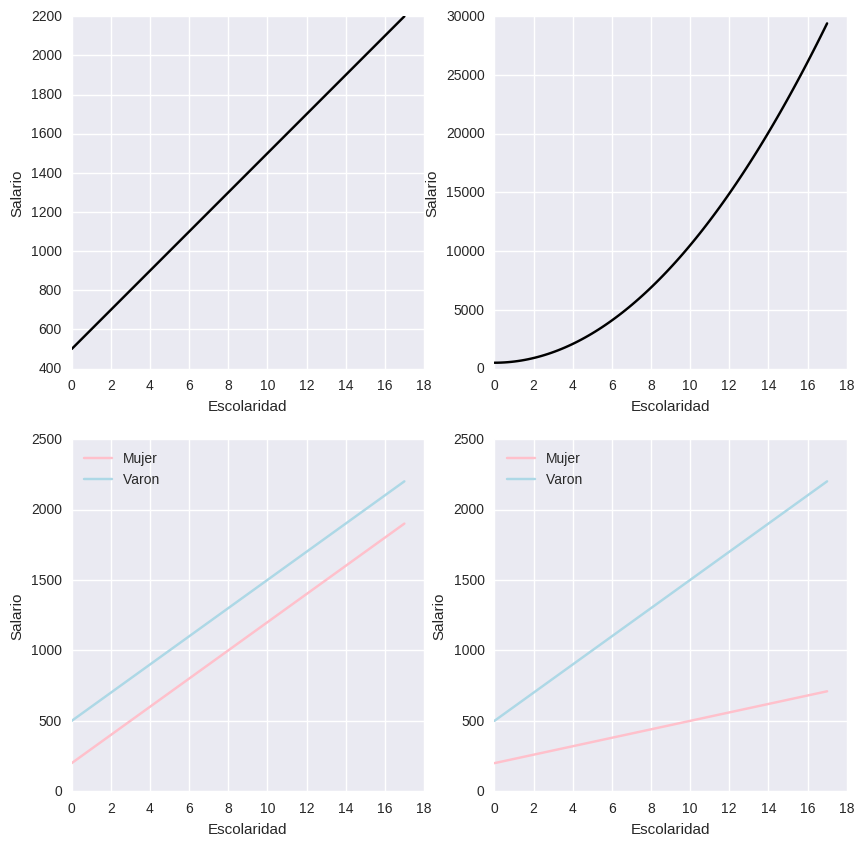
\includegraphics[scale = 0.5]{../img/capitulo2/modelo.png}
		\caption{En el gráfico se observa la relación lineal entre escolaridad y salario de modo que a mayor escolaridad mayor salario.En el gráfico se observa la relación lineal entre escolaridad y salario de modo que a mayor escolaridad mayor salario. Solo que los 2 años adicionales de escolaridad entre 14 y 16 implica un salario adicional de 5000 pesos mientras que los 2 años adicionales de 0 a 2 apenas marcan una diferencia.En el gráfico se observa la relación lineal entre escolaridad y salario de modo que a mayor escolaridad mayor salario tanto para varón como para mujer. Solo que la mujer parte de un salario inferior, pero aumenta al mismo ritmo con el aumento de la escolaridad. En el gráfico se observa la relación lineal entre escolaridad y salario de modo que a mayor escolaridad mayor salario tanto para varón como para mujer. Solo que la mujer además de partir de un salario inferior, aumenta a un ritmo diferente (menor) con el aumento de la escolaridad, lo cual amplía la brecha en los tramos superiores de escolaridad}
\end{figure}

De este modo podemos plantear que existe una relación \textit{linear} entre años de escolaridad y salario. De este modo cada año ofrece un retorno \textit{constante} de una determinada cantidad en moneda (en este caso nuestro parámetro a estimar $\beta$ estará en pesos). Esta es una de las limitaciones de esta metodología, que asume linearidad en los parámetros. Sin embargo, si suponemos que no es lo mismo un año de escolaridad universitaria que de primaria, es decir que existen retornos \textit{crecientes}, existe una manera de plantearlo sin violar los supuestos del modelo. Haciendo una transformación logarítmica del regresando, podemos plantear este escenario:

$$log(Y) = w_0 + \beta AE [2]$$

En este caso, nuestro parámetro a estimar estaría ya no en moneda sino en porcentajes. Es decir, un año más de escolaridad implicaría tanto más por ciento con lo cual cada año ofrece un retorno \textit{mayor en pesos} que el anterior.




Ahora sí, podemos introducir el concepto de \textit{interacción}. Primero, podemos suponer que el sexo ($S$) es una variable que influye en el salario de las personas. De este modo podemos introducir dicha variable como regresor en el modelo para, por un lado, obtener un estimador de cuán influyente es y, por el otro, aislar su efecto del retorno de la escolaridad. Es una forma de controlar por esta variable. Así el modelo quería formulado por:
 
$$log(Y) = w_0 + \beta_1 AE + \beta_2 S [3]$$



Ahora, podemos plantear que esta relación entre escolaridad y salario puede ser diferente según estemos hablando de una mujer o un varón. Es decir, no solo que los salarios medios cambian según el sexo, sino que cada año de escolaridad le ofrece retornos diferentes según esa persona sea mujer o varón. Esto se puede plantear con un modelo con términos de interacción del siguiente modo:

$$log(Y) = w_0 + \beta_1 AE + \beta_2 S + \beta_3  S.AE [4] $$



Esto cambia la interpretación de los estimadores, fundamentalmente el parámetro de ordenada al origen ($w_0$ en nuestro caso). Originalmente en la especificación del modelo en [1] y [2], era entendido como un salario básico, un monto por debajo del cual nadie era remunerado, sin importar cuantos años de escolaridad tuviese. Es decir, significaba cuánto ganaba alguien con 0 años de escolaridad. Sin embargo en el modelo  de [3] esto cambia y pasa a ser el salario mínimo no de todos sino del \textit{caso testigo}, que en nuestro ejemplo es un trabajador varón años de escolaridad. Para las mujeres, la variable $S$ tomará valor $1$ y se adicionará (o restará, porque los parámetros pueden ser de signo negativo) $\beta_2$. 

Finalmente, para el modelo [4] se obtiene para las mujeres una nueva ordenada al origen como una nueva pendiente. Es decir, no solo las mujeres ganan diferente, sino que su relación con los años de escolaridad es de otro orden. Este es el rol que cumple el intercepto y así debe interpretarse el rol de la ordenada al origen y el caso testigo. Esto será de mucha utilidad en la especificación del modelo CAPECO.

\subsection{El modelo detrás del indice CAPECO} \label{cap2-modeloCapeco}

Para la construcción del CAPECO 2001 se tomó como base la EPH correspondiente al mes de octubre de 2001. El modelo que subyace al índice CAPECO intenta aproximar el ingreso a partir de las variables que la literatura considera determinantes y a su vez se encuentran presentes en el Censo: 

\begin{itemize}
	\item Sexo 
	\item Edad
	\item Región geográfica
	\item Condición de actividad
	\item Años de escolaridad aprobados
\end{itemize}

A partir de estas variables se modelizó en una única ecuación los incrementos porcentuales en los ingresos laborales debidos a un incremento marginal en los años de escolaridad a partir de una función continua con pendientes diferenciales por nivel educativo. Se asumió el supuesto simplificador de considerar la cantidad de horas de trabajo como una función endógena de los años de escolaridad (los otros modelos de capital humano consideran esta variable, pero no se encuentra en el Censo).

Finalmente se incluyerón las variables de sexo, edad y lugar de residencia como explicativas de los diferenciales de ingreso a través de un conjunto de 35 dummies que reflejan todas las
combinaciones posibles entre las tres variables, asumiendo que existen relaciones entre
éstas. Esta última alternativa fue la seleccionada por considerarse que las diferencias de
los ingresos entre sexos, por ejemplo, no son uniformes a través de las distintas regiones
geográficas \cite{indec2004}. Dado que en este trabajo el área bajo análisis es la AGBA, no utilizaremos el resto de las variables que atañe a la región.

$$Ln Y_n = Ln Y_0 + r1. Esc_1 + r2. Esc_2 + r3. Esc_3 + $$
$$ \beta_0 m35ymas GBA + \beta_1 v14a24 GBA+ \beta_2 m14a24GBA + $$
$$\beta_3. v25a34 GBA+ \beta_4. m25a34GBA + \cdots + \epsilon $$

donde:

\begin{itemize}
	\item $Y_0$ son los ingresos laborales para un varón con 0 años de escolaridad de 35 años y más que reside en GBA. Es el intercepto u ordenada al origen.
	\item $Esc_1$ es escolaridad primaria y puede asumir valores desde 1 a 7
	\item $Esc_2$ es escolaridad secundaria y puede asumir valores de 1 a 5
	\item $Esc_3$ es escolaridad superior y puede asumir valores de 1 a 5
	\item $m35ymasGBA$ es una \textit{dummy} que asume valor = 1 si es una mujer de 35 años y más que reside en GBA
	\item $v14a24GBA$ es una \textit{dummy} que asume valor = 1 si es un varón de 14 a 24 que reside en GBA y así sucesivamente con las restantes 33 variables \textit{dummy} que combinan el sexo con la edad y la región de residencia.
\end{itemize}

Este es el modelo subyacente al CAPECO y de por sí ya constituye una herramienta para aproximarse al ingreso del hogar. Sin embargo, los investigadores a cargo tomaron la decisión de construir un índice cuyos coeficientes se basen en este modelo. 

El índice CAPECO se construye de acuerdo a la siguiente fórmula:

$$ CAPECO = \frac{\displaystyle\sum_{i=1}^{n}(CP_i * VAE_i)}{\displaystyle\sum_{i=1}^{n}Aeq_i} $$

donde:
\begin{itemize}
	\item n: total de integrantes del hogar
	\item CP: condición de percepción (asume distintos valores según la condición de actividad, la edad, el sexo y el lugar de residencia)
	\item VAE: valor de los años de escolaridad invertidos en el mercado laboral
	\item Aeq: valor en unidades de adulto equivalente de cada integrante del hogar (varía de acuerdo al sexo y la edad, siguiendo una tabla de necesidades calóricas y nutricionales)
\end{itemize}


Para ello construye 3 coeficientes previamente enumerados (CP,VAE y Aeq), de los cuales solo los dos primeros surgen del modelo previamente explicitado. El último es un insumo que se toma directamente de otra fuente. Se denomina \textit{Adulto equivalente} y expresa las necesidades nutricionales y energéticas según edad y sexo, en base a las necesidades de una unidad de referencia: un adulto varón entre 30 y 60 años \cite{indec2016b}. Las mismas surgen de la Encuesta de Gastos de los Hogares (ENGHo). Para el CAPECO de 2001, se tomó el dato correspondiente a la ENGHO 1996/97. Estas tablas de equivalencias pueden consultarse en el Anexo \ref{tab:tableAE2001}.

En cambio, los otros dos coeficientes (\textit{CP} y \textit{VAE}) son producto del modelo que subyace al CAPECO. El \textit{Coeficiente de Percepción} (CP) toma como caso base o testigo a un individuo de sexo masculino de 35 años y más que reside en GBA y asume valor 1. El resto de los individuos se considerará en relación a éste, utilizando los coeficientes que acompañan a las \textit{dummy} para establecer las diferencias de sus ingresos con respecto a éste. Si las mujeres y los jóvenes tienen ingresos inferiores, estos coeficientes tendrán un signo negativo, es decir funcionarán como “penalidades” a aplicarse sobre el valor de los ingresos del testigo
con sus mismos años de escolaridad. En general, todos los perceptores tienen una “penalización” respecto de los ingresos que percibe el perceptor equivalente, lo cual significa que sus años de escolaridad se ven depreciados a causa de su edad, sexo y lugar de residencia \cite{indec2016b}. El coeficiente se calcula como la proporción del ingreso estimado por el modelo para ese grupo de edad y sexo, en comparación con el ingreso estimado por el modelo para el caso testigo (varón de 35 o más).Sus valores pueden consultarse en la tabla \ref{tab:tableCP2001}


El \textit{Valor de los Años de Escolaridad en el mercado laboral} (VAE) se determinó del siguiente modo: se asignó una base arbitraria de valor 7 para el nivel educativo primaria completa (es decir, 7 años de escolaridad aprobados). A partir de este valor índice, se realiza el mismo procedimiento comparativo, comparando las diferencias para cada año de escolaridad frente a esa base 7. Sus valores pueden consultarse en la tabla \ref{tab:tableVAE2001}
 
 	\section{Autocorrelación espacial}

	\section{Desafios metodológicos}
	
A continuación se enumeran algunos de los problemas y dificultades existentes con la metodología utilizada en este trabajo con el espíritu de explicitar sus problemas de modo que sean tomados en consideración en los análisis posteriores que se lleven a cabo.	

	\subsection{Inactivos con rentas}

Este modelo se sostiene fuertemente en el paradigma del capital humano y en la valorización de dicho capital en el mercado de trabajo. Por lo tanto, resulta inadecuado para aquellos que a pesar de no formar parte del mercado de trabajo de todos modos perciben algún tipo de ingreso monetario. Podría citarse como ejemplo paradigmático los/las estudiantes que se mudaron a centros urbanos con universidades, que viven solos/as o con otros/as estudiantes que no trabajan pero perciben una renta de sus familias. En estos casos el CAPECO imputa un valor 0. Lo mismo puede ser dicho para toda situación de inactivos que vivan de rentas. 

También se puede mencionar que existirá un problema en general para el caso de los inactivos. Si bien se puede esperar que aquellos capitales acumulados durante la etapa activa, persistan en el tiempo dando rendimientos en la etapa inactiva (de modo que le nivel educativo de la persona en cuestión sigue ofreciendo información significativa sobre su ingreso actual producto de las rentas acumuladas en el pasado), esta situación cambia sensiblemente de acuerdo a la condición de inactividad de esta persona. Si cobra o no jubilación, pensión, etc. Esto fue considerado en el modelo original del CAPECO con coeficientes de percepción diferenciales para estas situaciones, pero para el caso de 2010 presenta un problema.

	
	\subsection{Ausencia de información}
	
El formulario censal básico de 2010 (el que ofrece resultados para unidades espaciales micro) no recaba información sobre la condición de inactividad. De este modo no sabemos para cada observación si la condición de inactividad es tal debido a percepción de rentas, jubilación, pensión, etc. Esto hace que para el CAPECO 2010, los coeficientes de percepción sean diferentes y aún más insensibles antes la inactividad. Esto lleva a mayores niveles de error.
		
Otra información ausente en la cédula censal básica que tiene alto impacto en el nivel de ingreso de acuerdo al capital humano son la cantidad de horas trabajadas. Este escollo fue sorteado mediante el supuesto simplificador mencionado previamente de que la cantidad de horas también es una función de los años de escolaridad. Sin embargo, hemos decidido volver a mencionarlo para explicitar esta situación. Esto tiene potencial impacto en el tramo inferior de ingresos, dado que para altos niveles de escolaridad es de esperar que los/as activos/as lleven adelante una jornada laboral completa. Para aquellos/as que trabajan menos horas, la cantidad es determinante en su nivel de ingreso.  

Otra falta de información en el Censo es si dicho trabajo es registrado o no. Esto también tiene alto impacto en la estimación de ingresos, especialmente en el tramo inferior (dado que los años de escolaridad están relacionados con el tipo de trabajo realizado en términos de formalidad). 

Una última cuestión a mencionar en relación al Censo es la ausencia en el formulario básico del sector de actividad en el que se desempeñan los/as activos/as. Las productividades diferenciales de los diversos sectores tienen su correlato en el nivel de salarios del sector. Esto tiene un impacto en todo el espectro de ingreso, pero es de esperar que, a diferencia de los casos anteriores, afecte particularmente al tramo de ingresos medios y altos. Un caso con el máximo de años de escolaridad concebido en el índice CAPECO (17 años) puede tener niveles de ingresos muy disimiles en función del sector de actividad en el que se desempeñe, debido a la productividad y el nivel de salarios del mismo. Esto puede redundar en una subestimación de ingresos por parte del CAPECO. 

Se menciona el formulario básico ya que es el único que permite obtener resultados a escala microespacial. El formulario ampliado incorpora algunos de estos elementos (jubilación, tamaño del establecimiento, sector, etc.) pero solo arroja resultados a nivel departamental.

Existe una última limitación vinculada a información insuficiente en las fuentes utilizadas, esta vez en relación a la EPH. La EPH se basa en un diseño muestral con una estrategia de estratificación en diversas etapas. Para poder realizar estimaciones en una muestra de estas características, y obtener intervalos de confianza para dichas estimaciones, es indispensable contar con los vectores de probabilidad de inclusión de primer y segundo orden de cada una de las observaciones. Sin los mismos, no se pueden establecer dichos intervalos. La EPH sí cuenta con el vector de pesos, que es la inversa de la probabilidad de inclusión producto de toda las etapas. Estos pesos o ponderadores permiten obtener un estimador, pero no así los intervalos de confianza. 

Por último, existe la sospecha de subdeclaración de ingresos en la EPH, en especial por parte de los sectores de altos ingresos. Al mismo tiempo se imputan ingresos para muchos casos donde las personas encuestadas se niegan a informar los mismos al encuestador. La decisión en este trabajo fue tomar esas imputaciones y registros de ingresos como datos válidos. Pero se explicita que estas cuestiones pueden redundar en errores de estimación (puntualmente pueden implicar una subestimación por parte del modelo).
	
	\subsection{Outliers}
	
Los modelos de regresión lineales tienen como una de sus principales desventajas, la extrema sensibilidad a valores extremos u outliers. En el caso del ingreso, la distribución del mismo dista mucho de asemejarse a la distribución normal y presenta casos extremos, tanto en el tramo inferior como superior. Estos casos pueden influir en el análisis. Sin embargo, una cuidada estrategia de detección de outliers puede disminuir este impacto. La remoción de outliers puede ser justificada para el análisis de distribución del ingreso. Para los casos de ingreso extraordinariamente altos, los mismos representan una porción muy pequeña. En el caso de los muy bajos ingresos, se debe tener más cuidado  ya que la asimetría de la distribución hace representen una proporción algo mayor. Sin embargo, se puede plantear el interrogante sobre los hogares que registran nulos ingresos en un contexto de una aglomeración urbana como el AGBA. Un hogar con nula percepción de ingresos puede ser considerado una situación coyuntural que amerita no sea considerado en el análisis.  


	\subsection{Problema   de   la   Unidad   Espacial   Modificable   (PUEM) y base cartográfica}


Radios censales - Unidades gepgráficas modificables

	
	\section{Instrumentos computacionales}
	
El presente trabajo utiliza el software \textit{REDATAM} par extracción y procesamiento de datos censales. Redatam es el acrónimo de REcuperación de DATos para Áreas pequeñas por Microcomputador.  El programa utiliza una base de datos jerárquica comprimida, que se puede crear en R+SP y que contiene microdatos y/o información agregada con millones de registros de personas, viviendas, manzanas de ciudades o cualquier división administrativa de un país. Es posible definir, a partir de una base de datos, cualquier área geográfica de interés (desde manzanas de una ciudad) o combinaciones de esas áreas, crear nuevas variables, obtener varios tipos de tabulados y exportar salidas a otros softwares. Los datos de diferentes niveles geográficos pueden ser combinados jerárquicamente para crear variables agregadas, y los resultados pueden desplegarse en mapas desde Redatam o transferirse a un Sistema de Información Geográfica (SIG). Todas las versiones de Redatam han sido desarrolladas y mantenidas por el Centro Latinoamericano y Caribeño de Demografía (CELADE), que es la División de Población de la CEPAL. Sin embargo es necesario mencionar las limitaciones que tiene a la hora de implementar diferentes técnicas. El repertorio de técnicas a utilizar sobre datos censales se encuentra limitado a aquellas disponibles en el software. Por eso, técnicas como análisis factorial o clusters solo pueden realizarse por fuera de \textit{REDATAM} sobre datos agregados para las unidades espaciales disponibles en el software. 

Para procesamiento de la EPH se utilizo el lenguaje de programación \textit{Python}, un lenguaje de programación interpretado multiparadigma, ya que soporta orientación a objetos, programación imperativa y, en menor medida, programación funcional. Puntualmente en lo relacionado al modelo de regresión se utilizaron los paquetes de software de licencia libre \textit{Scikit-learn} y \textit{SciPy}. Estos paquetes permiten implementar técnicas de copmutación científica y machine learning en \textit{Python}. Puntualmente dentro de \textit{SciPy}, se encuentra el módulo \textit{Statsmodels} que permite implementar la técnica de regresión múltiple con ponderadores (Weighted Least Squares). La totalidad de este trabajo, los códigos fuentes para la descarga y procesamiento de datos, se encuentra documentada online con licencia libre en la plataforma \textit{GitHub} bajo el usuario \textit{alephcero}. Esto permite chequear y reproducir este trabajo en su totalidad.

Finalmente la cartografía y visualización de datos fue llevada adelante utilizando los paquetes de software \textit{QGIS} y la plataforma online \textit{CARTO}. \textit{QGIS} o \textit{Quantum GIS} es un Sistema de Información Geográfica (SIG) de código libre desarrollado por Fundación OSGeo y permite manejar formatos raster y vectoriales a través de las bibliotecas GDAL y OGR, así como bases de datos de diversos tipos. \textit{CARTO}  es una plataforma de computación en la nube de Software as a Service (SaaS) que proporciona herramientas SIG y de mapeo web para su visualización en un navegador web. Es un software de código abierto basado en el motor de bases de datos PostgreSQL  y su módulo para operaciones de SIG (PostGIS). 

